\label{sec:simulation}


\sheriff{} is a functional replacement for the \pthreads{} library
that extends it with two novel features: \emph{per-thread memory protection} (allowing each thread to track memory accesses
independently of each other thread's accesses) and optional
\emph{memory isolation} (allowing each thread to read and write memory
without interference from other threads). \sheriff{} works through a
combination of \emph{replacing threads by processes}~\cite{grace} and
\emph{page-level twinning and diffing}~\cite{dsm:munin,dsm:treadmarks}.

Replacing \pthreads{} with
processes is surprisingly inexpensive, especially on Linux where both
\pthreads{} and processes are invoked using the same underlying system
call. Process invocation can actually
outperform threads because operating systems initially assign threads to the invoking
CPU to maximize locality, while it spreads processes across all CPUs~\cite{grace}. To
achieve the effect of shared memory, \sheriff{} maps globals and the
heap into a shared region (Section~\ref{simulation:sharememory}). It
also intercepts the \texttt{pthread\_create} call and replaces it with
a process creation call (Section~\ref{sec:fileshare}).

Using processes to simulate threads has two key advantages. First,
converting threads to processes enables the use of
per-thread page protection, allowing \sheriff{} to track memory
accesses by different threads, a feature that \sheriffdetect{} uses in
its false sharing detection algorithm (Section~\ref{sec:falseshare}).
Second, it
isolates threads' memory accesses from each other. This isolation
ensures that threads do not update shared cache lines, and because each
process naturally has its own distinct set of cache lines this
eliminates false sharing: \sheriffprotect{} takes advantage of this
feature (Section~\ref{sec:patrol}). 

To maintain the shared-memory semantics of a multithreaded program,
\sheriff{} must periodically update the shared heap and globals so
that modifications become visible to other threads. \sheriff{} delays these updates
until synchronization points such as lock acquisition and release
(Section~\ref{simulation:syn}). However, \sheriff{} takes care to
update only the changed parts of each page (Section~\ref{sec:updatingsharedmemory}).

\subsection{Simulating a Shared Address Space}
\label{simulation:sharememory}

\begin{figure}[!t]
\centering
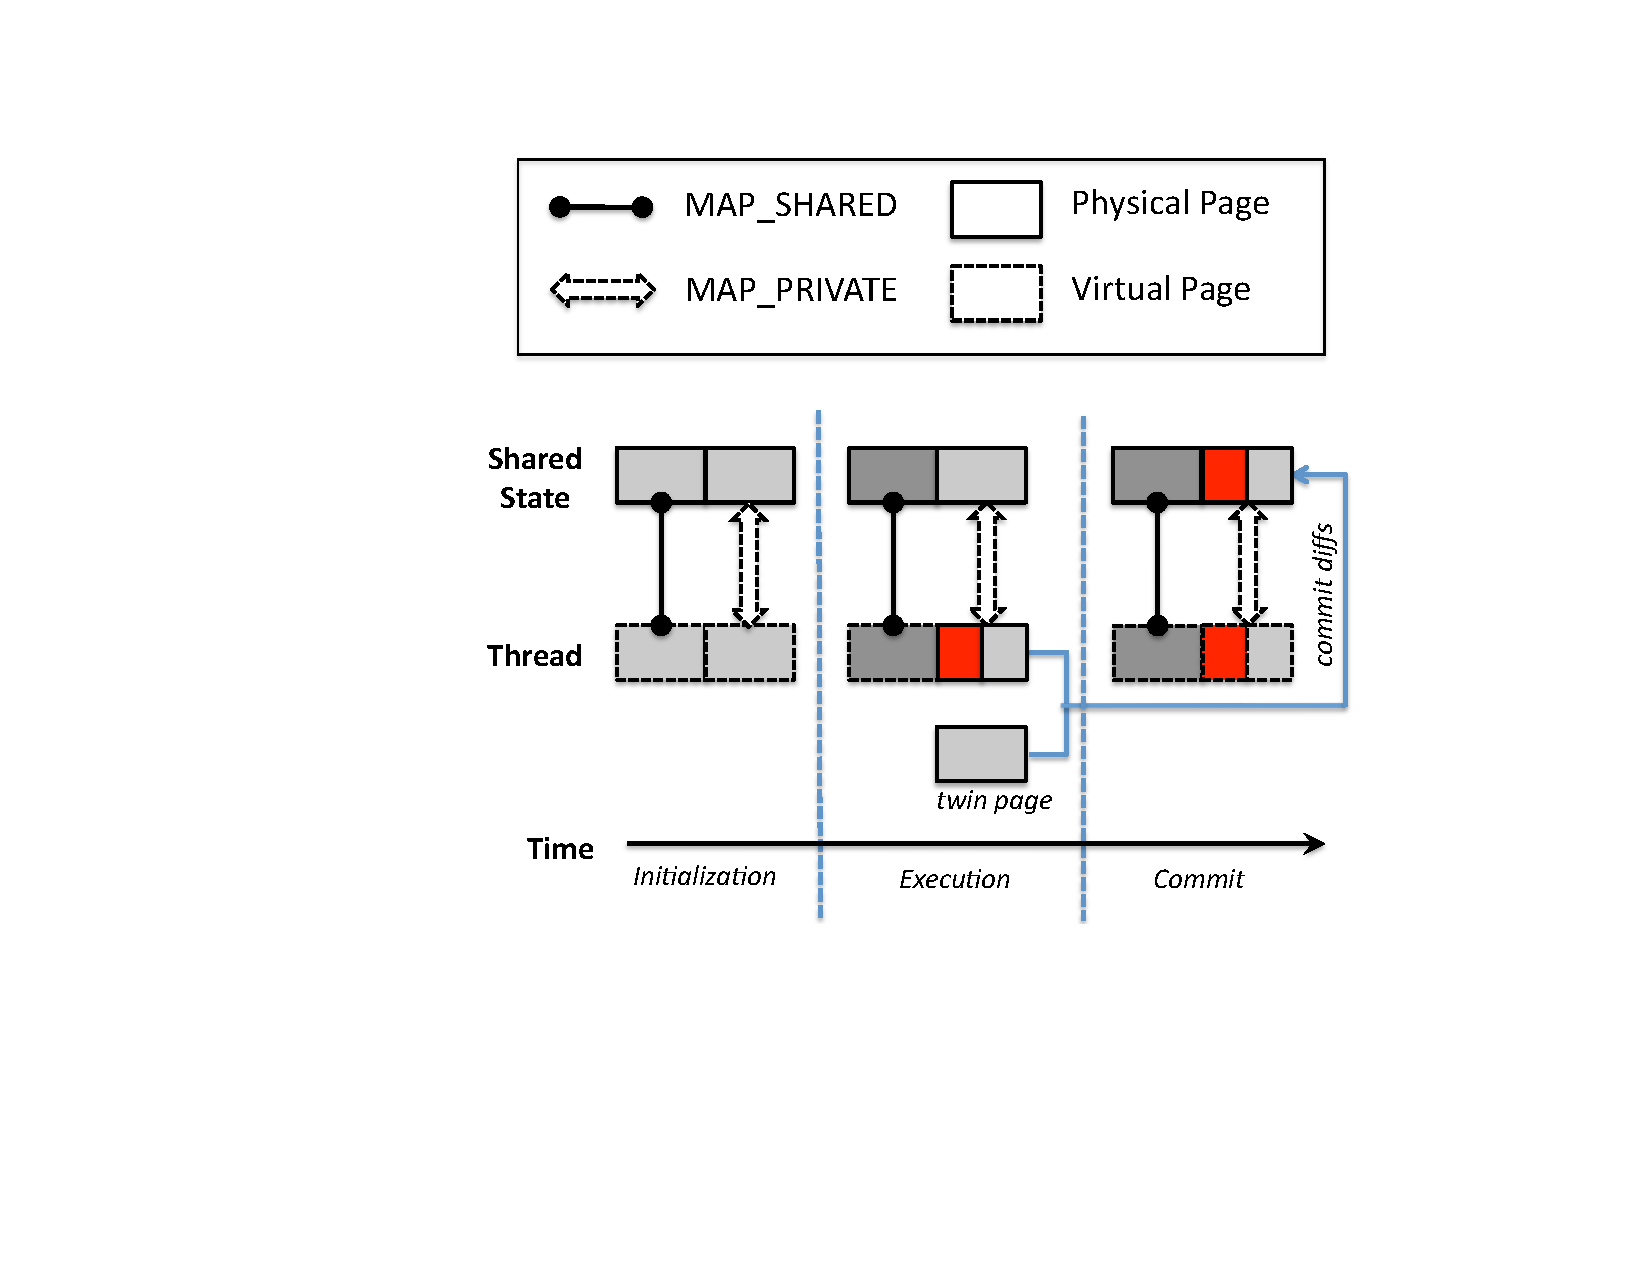
\includegraphics[width=3.5in]{figure/sheriffframework.pdf}
\caption{
\sheriff{} replaces \pthreads{} by simulating threads
with processes. It exposes an API that enables per-thread memory protection and memory isolation on a per-page basis. Each ``thread'' thus either operates directly
on shared memory, or on its own private
copy. For the latter, \sheriff{} commits diffs to shared mappings at synchronization
points (Section~\ref{simulation:syn}).
\label{fig:overview}}
\end{figure}

To create the effect of multi-threaded programs where
different threads share the same address space, \sheriff{} uses
memory mapped files to share the heap and globals across different
processes.  Note that \sheriff{} does not share the stack across
different processes because different threads have their own stacks
and, in general, multithreaded programs do not use the stack for cross-thread
communication.

\sheriff{} creates two different mappings for both the heap and the
globals.  One is a shared mapping, which is used to hold shared state.
The other is a private, copy-on-write (COW) per-process mapping that
each process works on directly.  Private mappings are linked to the
shared mapping through the one memory mapped file. Reads initially go
directly to the shared mapping, but after the first write operation,
both reads and writes are entirely private. \sheriff{}
updates the shared image at synchronization points, as described in
Section~\ref{simulation:thread}.

\sheriff{} uses a fixed-size mapping to hold
globals, which it checks to ensure is large enough to hold all
globals. \sheriff{} also uses a fixed-size mapping to store the heap
(by default, 1GB). Memory allocation requests from user
applications are satisfied from this fixed-size private mapping.

Since different threads allocate memory from this single fixed-size
mapping, the global superheap data structure is shared among different
threads and allocations are protected by one process-based mutex.  In
order to avoid false sharing induced by the memory allocator,
\sheriff{} employs a scalable ``per-thread'' heap organization that is
loosely based on Hoard~\cite{BergerMcKinleyBlumofeWilson:ASPLOS2000}
and built using HeapLayers~\cite{BergerZornMcKinley:2001}.  \sheriff{}
divides the heap into a fixed number of sub-heaps (currently 16).  The
metadata for each sub-heap is also shared by different threads and
protected by a cross-process mutex.  In order to reduce lock
contention, \sheriff{} assigns different sub-heaps to each thread at
creation time. Since each thread's heap allocates from different pages, 
the allocator itself is unlikely to collocate two objects from different 
threads on the same cache line.

Note that tools built with \sheriff{} can specify, on a per-page basis,
whether to use a shared mapping (so that updates are immediately
visible to other ``threads''), or a private mapping (so that updates
are delayed). Both \sheriffdetect{} and \sheriffprotect{} take
advantage of this facility.

\subsection{Shared File Access}
\label{sec:fileshare}

In multithreaded programs, all threads share the same file descriptor table
that tracks the process' open files.  For example, if one thread opens a 
file, the other threads see that the file has been opened.  However, 
multiple processes each have their own resources, including not only 
memory but also file handles, sockets, device handles, and windows.

While \sheriff{} could manage these directly, our current prototype
takes advantage of a feature of Linux that allows selective sharing of
memory and file descriptors. \sheriff{} sets the \texttt{CLONE\_FILES}
flag when creating new processes, resulting in child processes with
different address spaces but the same shared file descriptor table.

\subsection{Synchronization}
\label{simulation:syn}

\sheriff{} supports the full range of POSIX synchronization
operations (mutexes, conditional variables, barriers), as well as all
thread-related calls, including cancellation.

At each synchronization point, \sheriff{} must commit all changes made
by the current thread. The span between
synchronization points thus constitutes a single atomic
transaction. Note that \sheriff{}'s approach differs significantly
from previous transactional memory proposals~\cite{transaction},
including Grace. \sheriff{} is not optimistic, does not replace locks
with speculation (it actually acquires program-level locks), never
needs to roll back (it is always able to commit successfully), and
achieves low overhead for long transactions.

To simulate multithreaded synchronization, \sheriff{}
intercepts all synchronization object initialization function calls,
allocates new synchronization objects in a mapping shared
by all processes, and initializes them to be accessible by different
processes.

\sheriff{} wraps
all synchronization operations, including mutexes, condition
variables, and barriers in a similar fashion. For example, a call to
\texttt{pthread\_mutex\_lock} first ends the current transaction, 
then calls the corresponding \pthreads{} library function but on a
cross-process mutex. \sheriff{} then starts a new transaction after the
lock is acquired, which ends with the next synchronization operation.

Thread-related calls are implemented in terms of their process
counterparts. For example, \texttt{pthread\_join} ends the current
transaction and calls \texttt{waitpid} to wait for the appropriate
process to complete.


\subsection{Updating Shared Memory}

\label{sec:updatingsharedmemory}

At each synchronization point, \sheriff{} updates the shared
globals and heap with any updates that thread made.  To accomplish
this \sheriff{} uses \emph{twinning} and \emph{diffing}, mechanisms
first introduced in distributed shared memory systems to reduce
communication overhead~\cite{dsm:munin,dsm:treadmarks}.

% CC: Removed this, since diffs are always used to identify modifications
% \sheriffdetect{} uses diffs to identify modifications.

Figure~\ref{fig:overview} presents an overview of both mechanisms at
work. All private pages are
initially write-protected. Before any page is modified, \sheriff{}
copies its contents to a ``twin page'' and then unprotects the
page. At a synchronization point, \sheriff{} compares each twin page
to the modified page (byte by byte) to compute diffs.

\subsection{Example Execution}
\label{simulation:thread}

This section walks through an example of \sheriff{}'s execution from the start of a program to its termination.

% Figure~\ref{fig:overview} presents an overview of \sheriff{}'s execution.

\paragraph{Initialization: } Before the program begins, \sheriff{}
establishes the shared and local mappings for the heap and globals,
and initiates the first transaction.

\paragraph{Transaction Begin:}
At the beginning of every transaction, \sheriff{} write-protects any shared
pages so that later writes to these pages can be caught by
handling \texttt{SEGV} protection faults.  In later transactions,
\sheriff{} only write-protects pages dirtied in the last
transaction, since the others remain write-protected.

\paragraph{Execution: } While performing reads, \sheriff{} runs at
the same speed as a conventional multithreaded
program. However, the first write to a protected page triggers a page
fault that \sheriff{} handles.

\sheriff{} records the page holding the faulted address and then unprotects
this page so that future accesses run at
full speed.  Each page thus incurs at most one page fault per transaction.
Although protection faults and signals are expensive, these costs are
amortized over the entire transaction.

However, before servicing the fault, \sheriff{} must first obtain an
exact copy of this page (its twin). \sheriff{} accomplishes this by
forcing a copy-on-write operation on this page by writing to the start
of this page with contents from the same address (i.e., it
reads and writes the same value).

This step is essential to ensure that the twin is identical to the
original, unmodified page. After the signal handler, the OS's
copy-on-write mechanism creates a new, private page.

\paragraph{Transaction End: } At the end of each atomically-executed
region---at thread exit and before synchronization
points---\sheriff{} commits changes from
private pages to the shared space and reclaims memory holding old
private pages and twin pages.

\sheriff{} commits only the differences between the twin and the
modified pages. Once it has written these diffs, \sheriff{} issues an
\texttt{madvise} call with the \texttt{MADV\_DONTNEED} flag that
discards the physical pages backing both the private mapping and the
twin pages. This action allows the OS to reclaim this memory, helping
to ensure that \sheriff{}'s memory overhead remains close to that of
the original program.

\subsection{Discussion}

As Section~\ref{simulation:sharememory} notes, \sheriff{} does not
share the stack between different threads. When using \pthreads{},
threads are allowed to share stack variables with their parent.
As long as threads do not modify these variables,
\sheriff{} operates correctly. However, \sheriff{} does not preserve
\pthreads{} semantics for applications whose threads
\emph{modify} stack variables from their parent thread that their
parent then reads. Fortunately, passing stack variables to a thread
for modification is generally frowned upon, making it a rare coding
practice.

\sheriff{} cannot currently intercept atomic operations
written in assembly, so programs that implement their own
\emph{ad hoc} synchronization operations are not guaranteed to work
correctly (Xiong et al.\ have shown that 22--67\% of the uses of
\emph{ad hoc} synchronization they examined led to bugs or severe
performance issues~\cite{ad-hoc-considered-harmful}). We expect this
limitation to be less of a problem in the future because the
forthcoming C++0x standard exposes atomic operations in a standard
library, making it possible for \sheriff{} to intercept them.
